
%% bare_conf.tex
%% V1.4b
%% 2015/08/26
%% by Michael Shell
%% See:
%% http://www.michaelshell.org/
%% for current contact information.
%%
%% This is a skeleton file demonstrating the use of IEEEtran.cls
%% (requires IEEEtran.cls version 1.8b or later) with an IEEE
%% conference paper.
%%
%% Support sites:
%% http://www.michaelshell.org/tex/ieeetran/
%% http://www.ctan.org/pkg/ieeetran
%% and
%% http://www.ieee.org/

%%*************************************************************************
%% Legal Notice:
%% This code is offered as-is without any warranty either expressed or
%% implied; without even the implied warranty of MERCHANTABILITY or
%% FITNESS FOR A PARTICULAR PURPOSE! 
%% User assumes all risk.
%% In no event shall the IEEE or any contributor to this code be liable for
%% any damages or losses, including, but not limited to, incidental,
%% consequential, or any other damages, resulting from the use or misuse
%% of any information contained here.
%%
%% All comments are the opinions of their respective authors and are not
%% necessarily endorsed by the IEEE.
%%
%% This work is distributed under the LaTeX Project Public License (LPPL)
%% ( http://www.latex-project.org/ ) version 1.3, and may be freely used,
%% distributed and modified. A copy of the LPPL, version 1.3, is included
%% in the base LaTeX documentation of all distributions of LaTeX released
%% 2003/12/01 or later.
%% Retain all contribution notices and credits.
%% ** Modified files should be clearly indicated as such, including  **
%% ** renaming them and changing author support contact information. **
%%*************************************************************************


% *** Authors should verify (and, if needed, correct) their LaTeX system  ***
% *** with the testflow diagnostic prior to trusting their LaTeX platform ***
% *** with production work. The IEEE's font choices and paper sizes can   ***
% *** trigger bugs that do not appear when using other class files.       ***    
%                      ***
% The testflow support page is at:
% http://www.michaelshell.org/tex/testflow/



\documentclass[conference]{IEEEtran}
% Some Computer Society conferences also require the compsoc mode option,
% but others use the standard conference format.
%
% If IEEEtran.cls has not been installed into the LaTeX system files,
% manually specify the path to it like:
% \documentclass[conference]{../sty/IEEEtran}





% Some very useful LaTeX packages include:
% (uncomment the ones you want to load)


% *** MISC UTILITY PACKAGES ***
%
%\usepackage{ifpdf}
% Heiko Oberdiek's ifpdf.sty is very useful if you need conditional
% compilation based on whether the output is pdf or dvi.
% usage:
% \ifpdf
%   % pdf code
% \else
%   % dvi code
% \fi
% The latest version of ifpdf.sty can be obtained from:
% http://www.ctan.org/pkg/ifpdf
% Also, note that IEEEtran.cls V1.7 and later provides a builtin
% \ifCLASSINFOpdf conditional that works the same way.
% When switching from latex to pdflatex and vice-versa, the compiler may
% have to be run twice to clear warning/error messages.






% *** CITATION PACKAGES ***
%
\usepackage{cite}
% cite.sty was written by Donald Arseneau
% V1.6 and later of IEEEtran pre-defines the format of the cite.sty package
% \cite{} output to follow that of the IEEE. Loading the cite package will
% result in citation numbers being automatically sorted and properly
% "compressed/ranged". e.g., [1], [9], [2], [7], [5], [6] without using
% cite.sty will become [1], [2], [5]--[7], [9] using cite.sty. cite.sty's
% \cite will automatically add leading space, if needed. Use cite.sty's
% noadjust option (cite.sty V3.8 and later) if you want to turn this off
% such as if a citation ever needs to be enclosed in parenthesis.
% cite.sty is already installed on most LaTeX systems. Be sure and use
% version 5.0 (2009-03-20) and later if using hyperref.sty.
% The latest version can be obtained at:
% http://www.ctan.org/pkg/cite
% The documentation is contained in the cite.sty file itself.






% *** GRAPHICS RELATED PACKAGES ***
%
\ifCLASSINFOpdf
   \usepackage[pdftex]{graphicx}
   \usepackage{caption}
   \usepackage{subcaption}
   \usepackage{floatrow}
   \newfloatcommand{capbtabbox}{table}[][\FBwidth]
  % declare the path(s) where your graphic files are
  % \graphicspath{{../pdf/}{../jpeg/}}
  % and their extensions so you won't have to specify these with
  % every instance of \includegraphics
  % \DeclareGraphicsExtensions{.pdf,.jpeg,.png}
\else
  % or other class option (dvipsone, dvipdf, if not using dvips). graphicx
  % will default to the driver specified in the system graphics.cfg if no
  % driver is specified.
  % \usepackage[dvips]{graphicx}
  % declare the path(s) where your graphic files are
  % \graphicspath{{../eps/}}
  % and their extensions so you won't have to specify these with
  % every instance of \includegraphics
  % \DeclareGraphicsExtensions{.eps}
\fi
% graphicx was written by David Carlisle and Sebastian Rahtz. It is
% required if you want graphics, photos, etc. graphicx.sty is already
% installed on most LaTeX systems. The latest version and documentation
% can be obtained at: 
% http://www.ctan.org/pkg/graphicx
% Another good source of documentation is "Using Imported Graphics in
% LaTeX2e" by Keith Reckdahl which can be found at:
% http://www.ctan.org/pkg/epslatex
%
% latex, and pdflatex in dvi mode, support graphics in encapsulated
% postscript (.eps) format. pdflatex in pdf mode supports graphics
% in .pdf, .jpeg, .png and .mps (metapost) formats. Users should ensure
% that all non-photo figures use a vector format (.eps, .pdf, .mps) and
% not a bitmapped formats (.jpeg, .png). The IEEE frowns on bitmapped formats
% which can result in "jaggedy"/blurry rendering of lines and letters as
% well as large increases in file sizes.
%
% You can find documentation about the pdfTeX application at:
% http://www.tug.org/applications/pdftex





% *** MATH PACKAGES ***
%
\usepackage{amsmath, amsthm, amssymb, bm}
\usepackage{nicefrac}
% A popular package from the American Mathematical Society that provides
% many useful and powerful commands for dealing with mathematics.
%
% Note that the amsmath package sets \interdisplaylinepenalty to 10000
% thus preventing page breaks from occurring within multiline equations. Use:
%\interdisplaylinepenalty=2500
% after loading amsmath to restore such page breaks as IEEEtran.cls normally
% does. amsmath.sty is already installed on most LaTeX systems. The latest
% version and documentation can be obtained at:
% http://www.ctan.org/pkg/amsmath

\usepackage{enumerate}
\usepackage{enumitem}

% *** SPECIALIZED LIST PACKAGES ***
%
\usepackage{algorithm, algpseudocode}
% algorithmic.sty was written by Peter Williams and Rogerio Brito.
% This package provides an algorithmic environment fo describing algorithms.
% You can use the algorithmic environment in-text or within a figure
% environment to provide for a floating algorithm. Do NOT use the algorithm
% floating environment provided by algorithm.sty (by the same authors) or
% algorithm2e.sty (by Christophe Fiorio) as the IEEE does not use dedicated
% algorithm float types and packages that provide these will not provide
% correct IEEE style captions. The latest version and documentation of
% algorithmic.sty can be obtained at:
% http://www.ctan.org/pkg/algorithms
% Also of interest may be the (relatively newer and more customizable)
% algorithmicx.sty package by Szasz Janos:
% http://www.ctan.org/pkg/algorithmicx




% *** ALIGNMENT PACKAGES ***
%
%\usepackage{array}
% Frank Mittelbach's and David Carlisle's array.sty patches and improves
% the standard LaTeX2e array and tabular environments to provide better
% appearance and additional user controls. As the default LaTeX2e table
% generation code is lacking to the point of almost being broken with
% respect to the quality of the end results, all users are strongly
% advised to use an enhanced (at the very least that provided by array.sty)
% set of table tools. array.sty is already installed on most systems. The
% latest version and documentation can be obtained at:
% http://www.ctan.org/pkg/array


% IEEEtran contains the IEEEeqnarray family of commands that can be used to
% generate multiline equations as well as matrices, tables, etc., of high
% quality.




% *** SUBFIGURE PACKAGES ***
%\ifCLASSOPTIONcompsoc
%  \usepackage[caption=false,font=normalsize,labelfont=sf,textfont=sf]{subfig}
%\else
%  \usepackage[caption=false,font=footnotesize]{subfig}
%\fi
% subfig.sty, written by Steven Douglas Cochran, is the modern replacement
% for subfigure.sty, the latter of which is no longer maintained and is
% incompatible with some LaTeX packages including fixltx2e. However,
% subfig.sty requires and automatically loads Axel Sommerfeldt's caption.sty
% which will override IEEEtran.cls' handling of captions and this will result
% in non-IEEE style figure/table captions. To prevent this problem, be sure
% and invoke subfig.sty's "caption=false" package option (available since
% subfig.sty version 1.3, 2005/06/28) as this is will preserve IEEEtran.cls
% handling of captions.
% Note that the Computer Society format requires a larger sans serif font
% than the serif footnote size font used in traditional IEEE formatting
% and thus the need to invoke different subfig.sty package options depending
% on whether compsoc mode has been enabled.
%
% The latest version and documentation of subfig.sty can be obtained at:
% http://www.ctan.org/pkg/subfig




% *** FLOAT PACKAGES ***
%
%\usepackage{fixltx2e}
% fixltx2e, the successor to the earlier fix2col.sty, was written by
% Frank Mittelbach and David Carlisle. This package corrects a few problems
% in the LaTeX2e kernel, the most notable of which is that in current
% LaTeX2e releases, the ordering of single and double column floats is not
% guaranteed to be preserved. Thus, an unpatched LaTeX2e can allow a
% single column figure to be placed prior to an earlier double column
% figure.
% Be aware that LaTeX2e kernels dated 2015 and later have fixltx2e.sty's
% corrections already built into the system in which case a warning will
% be issued if an attempt is made to load fixltx2e.sty as it is no longer
% needed.
% The latest version and documentation can be found at:
% http://www.ctan.org/pkg/fixltx2e


%\usepackage{stfloats}
% stfloats.sty was written by Sigitas Tolusis. This package gives LaTeX2e
% the ability to do double column floats at the bottom of the page as well
% as the top. (e.g., "\begin{figure*}[!b]" is not normally possible in
% LaTeX2e). It also provides a command:
%\fnbelowfloat
% to enable the placement of footnotes below bottom floats (the standard
% LaTeX2e kernel puts them above bottom floats). This is an invasive package
% which rewrites many portions of the LaTeX2e float routines. It may not work
% with other packages that modify the LaTeX2e float routines. The latest
% version and documentation can be obtained at:
% http://www.ctan.org/pkg/stfloats
% Do not use the stfloats baselinefloat ability as the IEEE does not allow
% \baselineskip to stretch. Authors submitting work to the IEEE should note
% that the IEEE rarely uses double column equations and that authors should try
% to avoid such use. Do not be tempted to use the cuted.sty or midfloat.sty
% packages (also by Sigitas Tolusis) as the IEEE does not format its papers in
% such ways.
% Do not attempt to use stfloats with fixltx2e as they are incompatible.
% Instead, use Morten Hogholm'a dblfloatfix which combines the features
% of both fixltx2e and stfloats:
%
% \usepackage{dblfloatfix}
% The latest version can be found at:
% http://www.ctan.org/pkg/dblfloatfix




% *** PDF, URL AND HYPERLINK PACKAGES ***
%
\usepackage{url}
% url.sty was written by Donald Arseneau. It provides better support for
% handling and breaking URLs. url.sty is already installed on most LaTeX
% systems. The latest version and documentation can be obtained at:
% http://www.ctan.org/pkg/url
% Basically, \url{my_url_here}.




% *** Do not adjust lengths that control margins, column widths, etc. ***
% *** Do not use packages that alter fonts (such as pslatex).         ***
% There should be no need to do such things with IEEEtran.cls V1.6 and later.
% (Unless specifically asked to do so by the journal or conference you plan
% to submit to, of course. )


% correct bad hyphenation here
\hyphenation{op-tical net-works semi-conduc-tor}


\begin{document}
%
% paper title
% Titles are generally capitalized except for words such as a, an, and, as,
% at, but, by, for, in, nor, of, on, or, the, to and up, which are usually
% not capitalized unless they are the first or last word of the title.
% Linebreaks \\ can be used within to get better formatting as desired.
% Do not put math or special symbols in the title.
\title{Backtracking Re-agglomeration for\\
Community Detection in Dynamic Graphs}


% author names and affiliations
% use a multiple column layout for up to three different
% affiliations
\author{\IEEEauthorblockN{Pushkar Godbole}
\IEEEauthorblockA{College of Computing\\
Georgia Institute of Technology\\
Atlanta, Georgia 30332\\
pushkar.godbole@gatech.edu}
\and
\IEEEauthorblockN{Jason Riedy}
\IEEEauthorblockA{College of Computing\\
Georgia Institute of Technology\\
Atlanta, Georgia 30332\\
jason.riedy@cc.gatech.edu}
\and
\IEEEauthorblockN{David Bader}
\IEEEauthorblockA{College of Computing\\
Georgia Institute of Technology\\
Atlanta, Georgia 30332\\
bader@cc.gatech.edu}}

% conference papers do not typically use \thanks and this command
% is locked out in conference mode. If really needed, such as for
% the acknowledgment of grants, issue a \IEEEoverridecommandlockouts
% after \documentclass

% for over three affiliations, or if they all won't fit within the width
% of the page, use this alternative format:
% 
%\author{\IEEEauthorblockN{Michael Shell\IEEEauthorrefmark{1},
%Homer Simpson\IEEEauthorrefmark{2},
%James Kirk\IEEEauthorrefmark{3}, 
%Montgomery Scott\IEEEauthorrefmark{3} and
%Eldon Tyrell\IEEEauthorrefmark{4}}
%\IEEEauthorblockA{\IEEEauthorrefmark{1}School of Electrical and Computer 
%Engineering\\
%Georgia Institute of Technology,
%Atlanta, Georgia 30332--0250\\ Email: see 
%http://www.michaelshell.org/contact.html}
%\IEEEauthorblockA{\IEEEauthorrefmark{2}Twentieth Century Fox, Springfield, 
%USA\\
%Email: homer@thesimpsons.com}
%\IEEEauthorblockA{\IEEEauthorrefmark{3}Starfleet Academy, San Francisco, 
%California 96678-2391\\
%Telephone: (800) 555--1212, Fax: (888) 555--1212}
%\IEEEauthorblockA{\IEEEauthorrefmark{4}Tyrell Inc., 123 Replicant Street, Los 
%Angeles, California 90210--4321}}




% use for special paper notices
%\IEEEspecialpapernotice{(Invited Paper)}




% make the title area
\maketitle
% As a general rule, do not put math, special symbols or citations
% in the abstract
\begin{abstract}
In this paper, we present a streaming algorithm for agglomerative clustering, 
based on \emph{Modularity} maximization for community detection in evolving 
graphs. We employ a backtracking strategy to selectively and consistently 
reverse clustering in regions of the graph affected by incoming changes. 
Selective backtracking and re-agglomeration eliminates the need to re-initiate 
clustering as the graph evolves, thus reducing the computation cost and the 
\emph{Size of Change} in transitioning across community structures. In the 
experimental analysis of both typical and pathological cases, we evaluate and 
justify various backtracking and agglomeration strategies in context of the 
graph structure and incoming stream topologies. Evaluation of the algorithm on 
social network datasets, including Facebook (SNAP) and PGP Giant Component 
networks shows significantly improved performance over its 
conventional static counterpart in terms of execution time, \emph{Modularity} 
and \emph{Size of Change}.
\end{abstract}

% no keywords




% For peer review papers, you can put extra information on the cover
% page as needed:
% \ifCLASSOPTIONpeerreview
% \begin{center} \bfseries EDICS Category: 3-BBND \end{center}
% \fi
%
% For peerreview papers, this IEEEtran command inserts a page break and
% creates the second title. It will be ignored for other modes.
\IEEEpeerreviewmaketitle



\section{Introduction}
% no \IEEEPARstart
Community detection is one of the most critical aspects of
graph analysis, having primal applications in a wide variety of fields ranging
from molecular biology to social networks. However, due to the NP-hard nature
of the problem \cite{for} and arbitrary nature of the objective, deterministic
identification of the optimal community structure is rendered practically 
impossible, for large (real-world) datasets. Hence many approximation
algorithms and approaches have been developed to achieve near optimal
clustering. Since many (contemporary) networks are 
not static but rather evolve over time, the static approaches are rendered 
inappropriate for clustering of dynamic graphs. Dynamic community detection 
however has remained a largely untrodden field aside from the recent research 
 interest in the domain \cite{gor, ngu, hop, rie}, particularly in context of 
social networks.
\subsection{Contribution}
In this work, we build upon our previous dynamic community detection 
algorithm based on memoryless localized vertex-freeing \cite{rie} and present a 
backtracking re-agglomerative clustering approach inspired from the dGlobal BT
algorithm by Gorke et al. \cite{gor}. We test and evaluate the advantages and 
limitations of various agglomeration and backtracking strategies for the 
algorithm in context of \emph{snapshot quality} (\emph{Modularity}), 
\emph{history cost} (Size of Change) and computation cost \cite{cha} for 
different streaming graph topologies. We show that a fast, consistent 
and good quality clustering is possible by recursively storing and 
updating the historical community structure as a dendogram, with significantly 
lesser computation cost in terms of backtracking and agglomeration, 
over the dGlobal BT algorithm by Gorke et al. \cite{gor}.
\subsection{Nomenclature}
We use the standard graph theoretic notations to represent graph properties 
through out the paper \cite{for}. $G(V, E)$ represents a graph with $V$ 
representing the set of vertices and $E$ the set of edges. $|V| = n$ and $|E| = 
m$. \emph{Modularity} is represented by $Q$ and \emph{Size of Change} by 
$SoC$.\\
The terms, community detection, graph partitioning, clustering, have been 
interchangeably used to mean mapping of the vertices of $G$ into $\mathcal{C}$ 
($V \rightarrow \mathcal{C}$), where $\mathcal{C} = \{C_1, C_2, ..., C_p\}$ is 
a set of communities/partitions/clusters of vertices of $G$, such that for each 
$v \in V$, $v \in C_i$, for exactly one $i \in [1, p]$. Vertices 
representing agglomerations of multiple vertices into a single community are 
referred to as `community vertices'. The \emph{size(C)} of a community node $C$, 
refers to the number of vertices held by $C$. Community vertices with $size = 
1$ are referred to as `singletons' or `singleton communities'. 
\subsection{Outline}
Various metrics such as mutuality, conductance, betweenness have been employed, 
\emph{modularity} being the most widely accepted one, to evaluate the quality of 
graph partitioning. These metrics, although very efficient, are significantly 
dependent upon the structure and size of the graph, thus making the clustering 
of dynamic graphs very challenging. The objective of our re-agglomeration 
algorithm is maximizing/maintaining \emph{modularity} and minimizing \emph{Size 
of Change} (defined later) in transitioning from an old community structure to 
the new, in progressively transforming graphs. The next section discusses the 
past work related to dynamic community detection, specifically in context 
of \emph{Modularity} maximization. Section III introduces the metrics, 
\emph{modularity} and \emph{Size of Change}, and their dynamic charasterics and 
limitations in context of evolving graphs. Section IV describes our dynamic 
clustering algorithm with normative analysis of the backtracking and 
agglomeration strategies. Section V illustrates the performance of the algorithm 
on social network graph streams. Finally Section VI concludes the study with 
sound recommendations and direction of future work.
\section{Related Work}
Traditionally, the problem of static graph clustering has been widely studied, 
in context of \emph{modularity} optimization and beyond. The traditional methods 
of static graph clustering based on \emph{Graph Partitioning}, 
\emph{Partitional Clustering} and \emph{Spectral Clustering} rely on a 
pre-specified cluster count and/or cluster size. \cite{for}. These techniques 
render themselves unsuitable specifically in context of evolving graphs since 
the community structure of such graph also dynamically evolves with incoming 
changes, precluding the pre-specfication of such parameters. The 
\emph{Hierarchical Clustering} techniques on the other hand prove suitable in 
case of dynamic graphs due to their localized and emergent nature. These 
methods work by either starting from individual vertices and merging them into 
communities that improve the community structure of partitioning (Agglomerative) 
or by starting from a single large community and splitting it into 
smaller communities that yield a strong community structure (Divisive). Another 
class of methods for clustering of evolving networks, such as label propagation 
\cite{har}, relies on local information and connectivity patterns instead of 
using global metrics.  Our focus however is on agglomerative methods that 
optimize a numerical metric like \emph{modularity}. Following the seminal work 
on \emph{modularity} based greedy agglomerative clustering by Newman and Girvan 
\cite{new}, many modifications and improvements in the algorithm have since been 
achieved to improve the speed and performance of agglomerative clustering in 
static graphs \cite{cla, blo, sch, rie2}.\\
On the other hand, community detection in dynamic graphs has remained a 
relatively untouched field. The first work in this field by Hopcroft et al. 
\cite{hop} tracks the evolution of a graph by running agglomerative 
clustering on timely snapshots of the graph. This agglomeration however is 
memoryless and hence does not come under the class of dynamic clustering 
techniques. Gorke et al. \cite{gor2} introduce a partial ILP based technique for 
dynamic graph clustering with low difference updates, however this method proves 
unsuitable for large changes over time, due to its high computational 
requirement of solving the ILP. In our previous work, Riedy et al. \cite{rie} 
employ a localized vertex-freeing (to singletons), in affected regions of the 
graph and re-agglomerate from the intermediate partial clustering to yield a 
potentially higher \emph{modularity} community structure. Nguyen et al. 
\cite{ngu} also follow a similar approach of localized vertex-freeing around 
affected vertices and edges followed by their Quick Community Adaptation (QCA) 
algorithm to agglomerate the singleton vertices into suitable neighbors. 
Although these approaches yield very fast agglomeration algorithms, they tend to 
leave less flexibility for the clustering to sufficiently explore the solution 
space, on account of localized vertex-freeing. This may cause such methods to 
get trapped in local optima often due to larger communities sucking up smaller 
ones, referred to as the \emph{blackhole problem} \cite{jwu}. In this context, 
our backtracking algorithm allows consistent splitting of communities by storing 
and reverting past merges in affected regions of the graph and re-agglomerating 
thence. The dGlobal BT algorithm by Gorke et al. \cite{gor} employs a  
backtracking approach, very relevant to our algorithm. They conclude that their 
backtracking algorithm yields improved results in terms of \emph{modularity}, 
\emph{smoothness} and execution time over other algorithms. We expand on these 
previous works \cite{rie, gor} to develop and infer the most suitable 
backtracking and agglomeration strategy for dynamic community detection.
% \begin{itemize}
% \item \emph{Graph Partitioning}: These methods works by dividing the vertices of
% the graph into a predefined number of groups of predefined sizes by placing cuts
% in the graph that minimizes the cut-size (number of edges encountered by the
% cut).
% \item \emph{Partitional clustering}: Similar to graph partitioning, these 
% methods requires pre-specifying the number of communities for clustering and 
% then partitions the graph based on well-known techniques such as k-means 
% clustering.
% \item \emph{Spectral clustering}: These methods builds on top of the partitional
% clustering technique and apply similar partitioning methods to the 
% eigen-transformations of the graph.
% \item \emph{Agglomerative/Divisive clustering}: These methods are localized in 
% nature and work by either starting from individual vertics and merging them 
% into 
% communities that improve the community structure of partitioning 
% (Agglomerative) or by starting from a large connected component and splitting 
% it into components that yield a strong community structure (Divisive).
% The \emph{modularity} based re-agglomeration techniques comes under this 
% paradigm and 
% proves suitable for dynamic graphs, due to the non-requirement of 
% pre-specifying number and size of communities and localized nature of the 
% merge steps.
% \end{itemize}
\section{Preliminaries}
Graphs, particularly graphs representing real networks of objects, generally
exhibit a community structure. In other words, some regions of such graphs are
more closely connected than others. These closely knit groups in
graph-analytical context are called communities, wherein the graph has 
denser connections between the vertices within communities but sparse 
connections between vertices across communities. The metric of 
\emph{Modularity} coined by Newman and Girvan \cite{new}, is a widely used 
measure of the strength of partitioning, based on the premise that, a community 
structure would have collections of vertices more strongly connected internally 
than would occur from random chance.\\
In general, \emph{modularity} based agglomeration techniques start off by 
placing all graph vertices into singleton communities, recursively merging 
the communitiy vertices along edges, yielding an improvement in 
\emph{modularity}. 
The newly agglomerated graph formed from the merged vertices then acts as the 
starting point for the subsequent clustering, until no further improvement in 
\emph{modularity} is possible, thus reaching a local maximum.\\
In case of dynamic graphs, as the graph evolves (due to insertion and deletion 
of vertices and/or edges) the community structure and hence the 
\emph{modularity} evidently changes apropos. Modifying the partitioning to 
maximize/maintain \emph{modularity} entails creation and deletion of communities 
along with transitions of vertices between communities. Minimizing these 
transitions in an attempt to maximize \emph{modularity} ensures a smooth 
transition from an old partitioning to new. The \emph{Size of Change} metric, 
has been defined to quantify this change in partitioning w.r.t. vertex 
transfers.
\subsection{Modularity}
\label{Modularity}
Mathematically, \emph{Modularity} is defined as the fraction of the edges that 
fall within the given modules minus the expected value of such fraction if edges 
of the graph were distributed at random. Amongst the most commonly used methods 
to calculate \emph{modularity} and the one used here, the randomization of edges 
is based on the criterion that the degree of each vertex is preserved in the 
canonical random graph. For a graph G(V, E), with $n$ vertices and $m$ edges, 
we define $A_{ij}$ as the adjacency of vertices $i$ and $j$, i.e. $A_{ij} = 1$ 
if an edge exists between vertices $i$ and $j$ in G and 0 otherwise. Similarly, 
$P{ij}$ is defined as the expected number of edges between vertices $i$ and $j$ 
in the canonical random graph $R_G$. We define $\delta_{ij}$ as the community 
equivalence which is 1 if vertices $i$ and $j$ belong to the same community and 
0 otherwise. Then, based on this definition, the \emph{modularity}(Q) can be 
expressed as:
\begin{equation}
Q = \frac{1}{2m} \sum_{ij} (A_{ij} - P_{ij}) \delta_{ij} 
\end{equation}
The value of $P_{ij}$ can be computed using the randomization model in which
the degree of all vertices is kept intact and the connections changed. Graph G
with $m$ edges will have in all $2m$ stubs (half edges). For vertices $i$ and 
$j$,
their stubs can be connected to any of the remaining $2m - 2$ stubs. For large
value of $m$, $2m - 2 \approx 2m$. Therefore, the probability of having an edge
between $i$ and $j$ in $R_G$ would be given by $k_i/2m \times k_j/2m
= k_ik_j/4m^2$ making the expected number of edges, $P_{ij} = 2m \times
k_ik_j/4m^2 = k_ik_j/2m$ (where $k_i$ and $k_j$ are the degrees of vertics $i$
and $j$ in G and hence in $R_G$). Thus the above equation for
modularity can be simplified to:
\begin{equation}
Q = \frac{1}{2m} \sum_{ij} (A_{ij} - \frac{k_ik_j}{2m}) \delta_{ij}
\end{equation}

Notwithstanding its limitations, in particular w.r.t. the resolution 
limit \cite{for2}, modularity has certain properties that make it suitable for 
agglomerative clustering \cite{for, bran}:
\begin{itemize}
 \item For an undirected and unweighted graph G, the modularity Q lies between
the range $-1/2 \leqslant Q \leqslant 1$. A positive Q implies that, the
number of edges within communities exceeds the number expected on the basis of
$R_G$. The modularity of the entire graph as a single community is zero while
that of all singletons is negative
\item Isolated (degree 0) vertics have no impact on the modularity of a
community structure. Thus the optimal clustering for graphs $G(V_1, E_1)$ and 
$G'(V_1+V_2, E_1)$ would have equal optimal modularities, with all vertices 
from $V_2$ isolated into singleton communities.
\item In the clustering with maximum modularity, each connected component is a 
separate cluster. i.e. placing disconnected subgraphs of G, if they exist, in 
different clusters yields the highest modularity
\item Maximum modularity clustering is non-local: Changes to one 
region of the graph may propagate to the other regions, yielding a completely 
different optimal clustering
\end{itemize}
\subsection{Differential Modularity}
\label{diffmod}
One of the primary advantages of using Modularity as a metric for 
dynamic agglomeration is that, its computation is localized, in that it is 
possible to compute the contribution to the overall modularity by each 
individual community. The expression for the same is given by:
\begin{equation} \label{eq:3}
\Delta Q_C = \frac{E_C}{m} - \frac{Vol_C^2}{4m^2}
\end{equation}
Where $\Delta Q_C$ is the contribution to modularity by community $C$, $E_C$ is 
the number of internal edges in community $C$ and $Vol_C$ is the volume or the 
sum of the degrees of all vertices internal to community 
$C$. $m$ is the total number of edges in the original graph.\\
Most \emph{modularity} based agglomeration schemes prioritize merges based on 
their differential contribution to overall \emph{modularity}. However, merge 
along the highest $\Delta Q$ edge doesn't always guarantee a near-optimal 
community structure. Although \emph{modularity} serves as a good metric to 
evaluate pre-existing clustering, its not always very well suited to evaluate 
the best possible merges. This can mainly be attributed to the fact that the 
initial merges in the agglomeration are driven by the second term in equation
(\ref{eq:3}). The first term becomes dominant only after the vertices merge 
into 
non-singleton communities. Thus a best-merge-first technique initially prefers 
to merge along least volume edges, promoting the merge along bridge edges 
(edges connecting two communities), among others. The \emph{pair of 
n-wheels} graph in figure \ref{wheel10g} illustrates the impact of using a 
best-merge-first approach, yielding an additional bridge community shown in 
figure \ref{wheel10bf}, bringing down the modularity to 
$\frac{4n}{4n+1}-\frac{1}{2}-\frac{4n+21}{(4n+1)^2}$ from 
$\frac{4n}{4n+1}-\frac{1}{2}$, for the optimal clustering shown in figure 
\ref{wheel10o}. A best merge first agglomeration on a rectangular \emph{2D} 
lattice of such \emph{n-wheels} yields a highly suboptimal clustering 
populated heavily by bridge communities. The paper by Brandes et al. \cite{bran} 
illustrates another example using a \emph{regular 2-clique} graph showing 
how the worst possible clustering can manifest using a best-merge-first 
agglomeration strategy.\\
Secondly, given the $\Delta Q$ of the neighboring edges left in the wake of a 
merge changes after every merge, the complexity of the best-merge-first strategy 
goes to $O(mn)$ for an instance of agglomeration. Therefore, while the 
best-merge-first strategy affords good quality clustering in general, its 
relevance especially in the context of dynamic community detection is contingent 
upon the graph topology and computation cost considerations.
\begin{figure}
\begin{center}
\begin{subfigure}{0.45\textwidth}
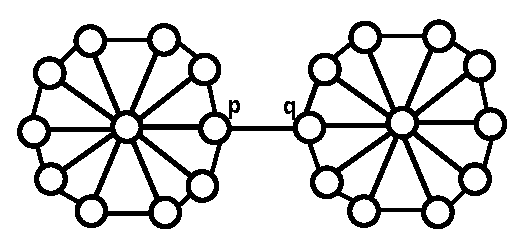
\includegraphics[width=\linewidth]{wheel10.pdf}
\caption{\emph{Pair of n-wheels} $(n=10)$} \label{wheel10g}
\end{subfigure}
\end{center}
\begin{subfigure}{0.45\textwidth}
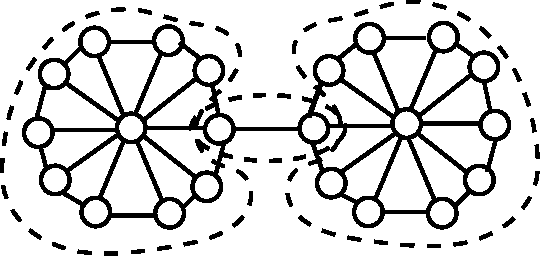
\includegraphics[width=\linewidth]{wheel10_bestfirst.pdf}
\caption{Best merge first clustering} \label{wheel10bf}
\end{subfigure}
%\hspace*{\fill} % separation between the subfigures
\begin{subfigure}{0.45\textwidth}
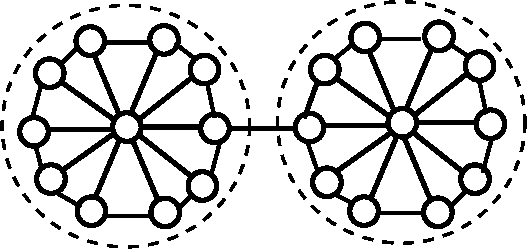
\includegraphics[width=\linewidth]{wheel10_optclust.pdf}
\caption{Optimal clustering} \label{wheel10o}
\end{subfigure}
\caption{\label{wheel10} Best merge first clustering in (a) prioritizes merge 
along bridge-edge \emph{(p, q)}, leading to suboptimal clustering (b) instead of 
(c) \emph{[Dashed lines represent clusters]}\vspace{-0.5cm}}
\end{figure}
\subsection{Size of Change}
The Size of Change metric needs to reflect the difference between two
 community structures based on the community associations of all vertices. 
However, since the communities do not have explicit tags, the measure for each 
node must be relative to the local change in terms of its neighborhood. This is 
done based on the following three measures of change for each node:
\begin{itemize}
 \item Nodes that were not in its community, but now are (Join)
 \item Nodes that were in its community, but now aren't (Leave)
 \item Nodes that were in its community and still are (Stay)
\end{itemize}
Based on these three changes, we define two parameters to quantify change in
the neighborhood of each node $(v)$:
\[c_J(v) = \frac{J(v)}{S(v) + J(v)}\]
\[c_L(v) = \frac{L(v)}{S(v) + L(v)}\]
Where $c_J(v)$ and $c_L(v)$ are the \emph{Join} and \emph{Leave} parameters
for $v$'s neighborhood. $J(v)$ is the number of neighbors that newly joined
$v$'s community, $L(v)$ the number of neighbors that left $v$'s community and 
$S(v)$ is the number of neighbors in $v$'s community that stayed unchanged. 
Based on $c_J(v) > mean(c_J(v)) + 2stddev(c_J(v))$ or $c_L(v) >
mean(c_L(v)) + 2stddev(c_L(v))$, we mark node $v$ as changed. The total number
of vertices that are marked as changed based on this criterion is finally
defined as the \emph{Size of Change (SoC)}.
\subsection{A case for Backtracking}
\label{caseforbt}
Dynamic aggomerative algorithms work by identifying affected community vertices 
(based on a chosen strategy) and modifying them for subsequent 
reagglomeration. However, there lies a fundamental difference between 
community vertices affected by edge insertion and deletion operations. In 
particular, edge insertions are forward looking changes that affect the 
subsequent community structure. But edge deletions on the other hand are 
backward looking, in the sense that they preclude the existing community 
structure. Conventional dynamic agglomeration techniques use vertex-freeing 
around affected regions of the graph, buy plucking out \emph{affected} vertices 
from communities and placing them in singleton communities. Consider for example 
the case of a change-batch that deletes edges from a community, splitting it 
into two disconnected subgraphs as shown in figure \ref{graph}.
\begin{figure}
\begin{subfigure}{0.45\textwidth}
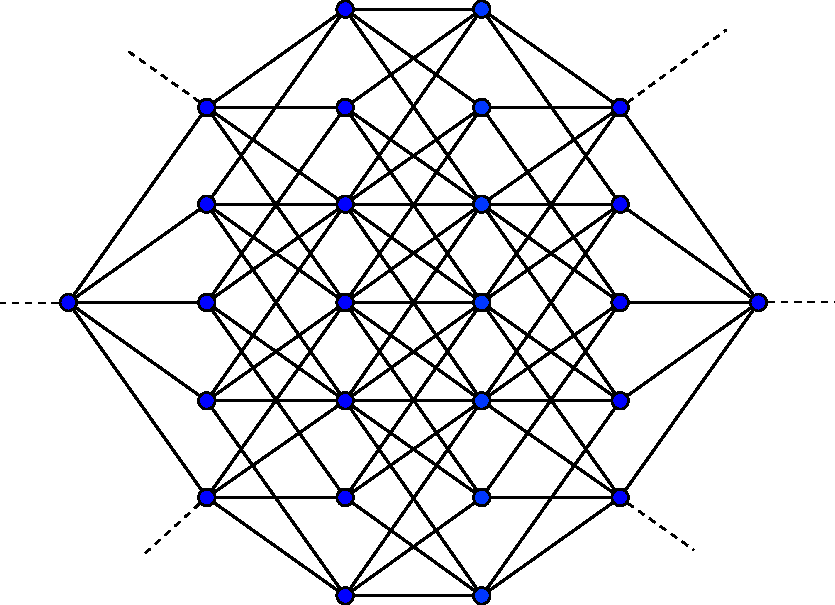
\includegraphics[width=\linewidth]{graph.pdf}
\caption{Initial graph community} \label{graph_init}
\end{subfigure}
\raisebox{8pt}{$\boldsymbol{\rightarrow}$}
%\hspace*{\fill} % separation between the subfigures
\begin{subfigure}{0.45\textwidth}
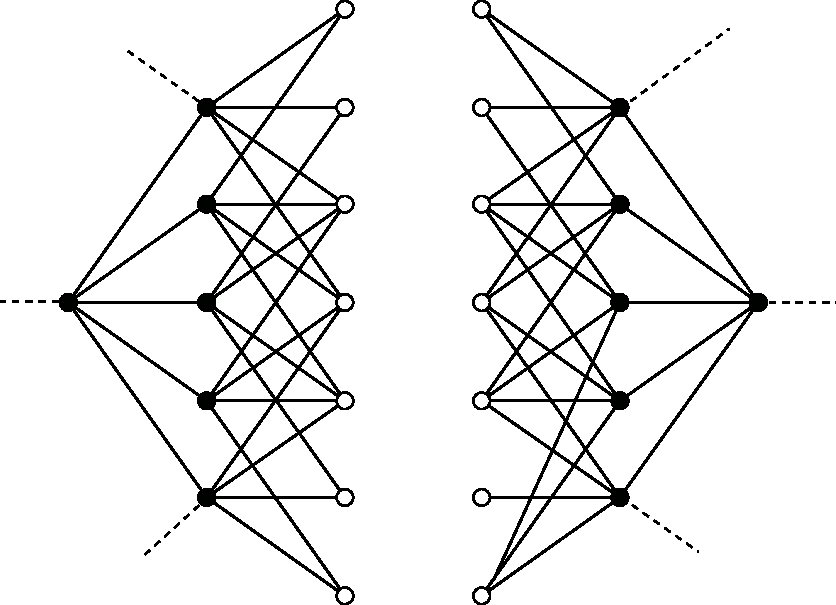
\includegraphics[width=\linewidth]{graph_split.pdf}
\caption{Updated graph community} \label{graph_split}
\end{subfigure}
\caption{\label{graph} As the graph transitions from (a) to (b), a conventional 
localized vertex-freeing strategy yields a suboptimal community structure where 
two disconnected subgraphs end up belonging to the same cluster. \emph{[Blue 
vertices lie in the same cluster $C$. White vertices become free 
singletons, that will likely re-join $C$ through the connecting edges, in 
subsequent agglomeration.]}\vspace{-0.5cm}}
\vspace{-0.2cm}
\end{figure}
A strict neighborhood based vertex-freeing strategy may only free vertices 
local to the affected edges, while other vertices (which must now ideally 
belong to two separate communities) are still tagged to the same community. A 
consistent backtracking strategy on the other hand is not restricted just to 
the neighborhood of the affected edges. It works by locally reverting the 
community structure by chronologically splitting community vertices to 
eliminate the now invalidated merges, reverting the community structure back to 
a point from where all the affected community vertices (not necessarily in the 
neighborhood) can re-evaluate their affiliations in the subsequent 
agglomeration.

\section{The Backtracking Re-agglomeration Algorithm}
Any dynamic agglomeration algorithm is primarily composed of two components. 
For each incoming batch of graph changes, the algorithm must execute the 
following two steps:
\begin{itemize}
 \item \textbf{Modification:} \emph{Identifying and reverting} affected 
regions of the community structure in response to the incoming graph change, to 
transform the past clustering $\mathcal{C}$ into a partial clustering 
$\mathcal{C'}$ to allow subsequent agglomeration, thus facilitating local 
exploration of the solution space.
\item \textbf{Re-agglomeration:} Given the partial clustering $\mathcal{C'}$, 
\emph{identifying and merging} the community vertices to reach a local optimum 
with 
a community structure potentially \emph{better} than the previous, in light of 
the graph change.
\end{itemize}
The graph changes in this context are restricted only to edge insertions and 
removals. Vertex insertions and removals have not been considered. However, it 
may be noted as presented in Section \ref{Modularity} that, newly added 
vertices can be considered to be part of a pre-existing \emph{rogue-vertex 
cloud ($V'$)}, disconnected from rest of the graph and each other, since such 
vertices dont affect \emph{modularity}. Therefore, this approach can be 
conveniently extended to vertex insertions and removals. A \emph{better} 
community structure in context of our algorithm is the one that yields a higer 
\emph{modularity}.\\
Similar to static agglomeration, the algorithm starts off by 
agglomerating singleton community vertices along edges that improve 
\emph{modularity}. But in addition to the present community structure, it also 
maintains a dendogram of the historical merges of all community vertices in 
time. 
For every incoming batch of edge changes, the algorithm splits the relevant 
communities either partially or completely based on the chosen 
\textit{backtracking strategy} described later, thus pruning/modifying the 
dendogram in the process. This is followed by a recursive update of the 
dendogram to reflect the inertion/remval of the edge. Finally, the algotithm 
merges community vertices along edges that improve \emph{modularity}. The order 
in 
which the community edges are considered for the merge is based on the 
\textit{agglomeration strategy}, discussed subsequently. 
\subsection{Backtracking}
Given the advantages of backtracking over the conventional 
 techniques such as vertex-freeing, as noted in Section 
\ref{caseforbt}, it is chosen as the community modification technique 
for our algorithm. The backtracking strategy defines how a batch of incoming 
edge changes is handled in the community dendogram of the graph. Broadly, the
backtracking strategies presented below are a combination of two methods: 
\emph{Edit Edge} and \emph{Split Community}.
\vspace{0.2cm}
\subsubsection{Backtracking Methods}
\label{btmethods}
\begin{itemize}
\vspace{0.2cm}
 \item \textbf{Edit Edge:} Keeps the community structure intact but 
recursively edits the underlying adjacency of the community vertices to change 
the weights of the edges. Editing the underlying adjacency requires 
knowledge of the chronological order in which the corresponding merges 
occurred. Figure \ref{dendo} illustrates an example of the adjacency 
induced by the existence of an edge DE in the base graph, on the subsequent 
community graph with the parent stacks for vertices D and E as shown in TABLE 
\ref{pstack}.

\begin{figure}
\begin{floatrow}
\ffigbox{%
  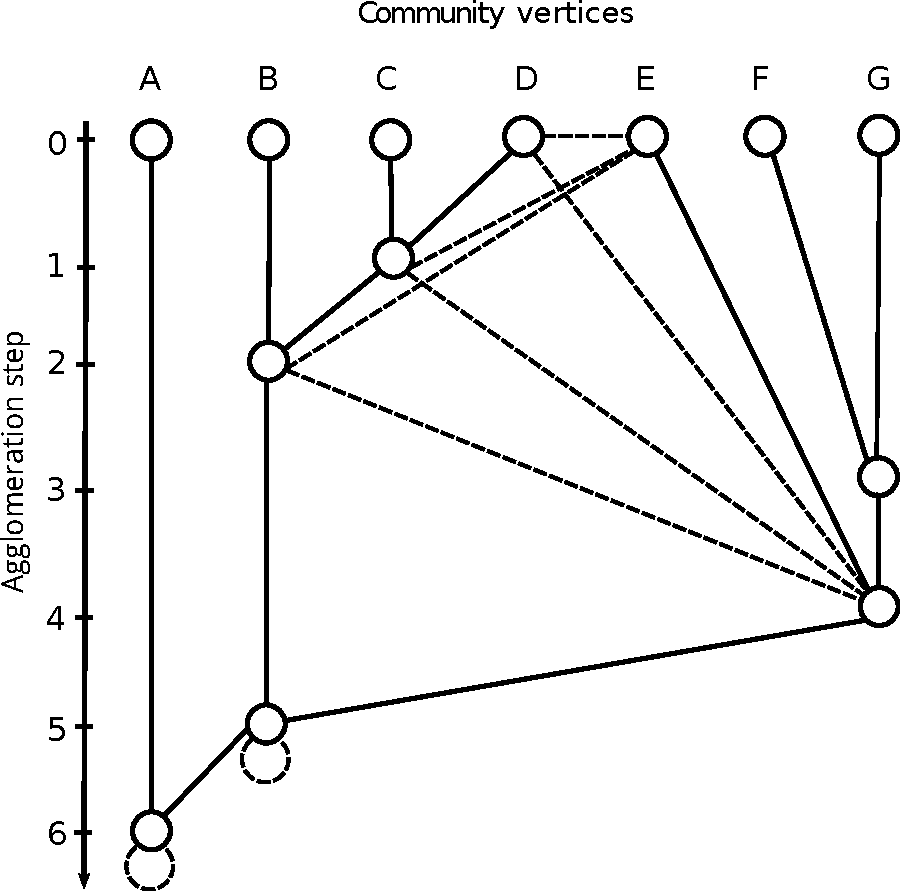
\includegraphics[width=4cm]{dendogram1.pdf}
}{%
  \caption{\label{dendo}}%
}
\hspace{1cm}
\capbtabbox{%
  \begin{tabular}{c|c}\hline
D & E\\\hline
C & \\\hline
B & \\\hline
  & G\\\hline
 & B\\\hline
A & A\\\hline
\end{tabular}
\vspace{1cm}
}{%
  \caption{\label{pstack}}%
}
\end{floatrow}
\vspace{0.3cm}
Figure \ref{dendo}: Dendogram of adjacency induced by base-edge DE\\
\flushleft TABLE \ref{pstack}: Parent stacks of vertices D, E
\vspace{-0.5cm}
\end{figure}
The solid lines in the dendogram represent the merges of community vertices 
as time progresses along the y-axis and the dashed lines represent the edges 
induced by the base edge on the community graph. The timestamps associated with 
these merges help determine the order of recursively editing the induced 
edges. In the above figure, deleting the edge DE in the base graph implies 
decrementing the weights of the induced edges AA, BB, GB, GC, GD, BE, CE, DE by 
the weight of the deleted base-edge DE in that order. The list of edges induced 
($IE_{ab}$) by base edge \emph{ab} can be generated from the parent stacks of 
$a$ and $b$ using Algorithm \ref{editedgealg}. Here $P_i(a)$ represents the 
$i^{th}$ parent of $a$, $a$ being the zeroth. $T_i(a)$ represents the timestamp 
of the $i^{th}$ merge of $a$.
\begin{algorithm}
\begin{algorithmic}
\State $i = size(P(a))$ //{ Size of parent stack of a}
\State $j = size(P(b))$ //{ Size of parent stack of b}
\While{$i!=0$ or $j!=0$}
  \State $IE_{ab} \gets (P_i(a), P_j(b))$
  \If{$T_i(a) > T_j(b)$}
    \State $k = j-1$
    \While{$P_i(a) != P_k(b)$ and $k > 0$}
      \State $IE_{ab} \gets (P_i(a), P_k(b))$
      \State $k \gets k-1$
    \EndWhile
    \State $i \gets i-1$
  \Else
    \State $k = i-1$
    \While{$P_k(a) != P_j(b)$ and $k > 0$}
      \State $IE_{ab} \gets (P_k(a), P_j(b))$
      \State $k \gets k-1$
    \EndWhile
    \State $j \gets j-1$
  \EndIf
\EndWhile
\end{algorithmic}
\caption{Induced Edges}
\label{editedgealg}
\end{algorithm}

\item \textbf{Split:} Splits a community into its two components, 
reversing the latest merge in the community dendogram. For instance, splitting 
community node A in Figure \ref{dendo} would be accomplished by subtracting the 
adjacency of node B from that of A and recursively reverting the parent stack 
of all vertices in community node B (B, C, D, E, F, G) by one (from A to B).
\end{itemize}
The three backtracking policies below define the \emph{extent of backtracking}, 
given an edge change \emph{ab}:
\begin{itemize}
 \item \textbf{Edit Edge:} Merely execute \emph{Edit Edge} for edge 
\emph{ab} keeping the community structure intact
 \item \textbf{Split to Separation:} Recursively \emph{Split} the community 
node containing edge \emph{ab} until vertices \emph{a} and \emph{b} belong to 
separate communities followed by \emph{Edit Edge}
 \item \textbf{Split to Singletons:} Recursively \emph{Split} the 
community 
vertices containing vertices \emph{a} and \emph{b}, until \emph{a} and \emph{b} 
both become singleton communities followed by \emph{Edit Edge}
\end{itemize}
Note that \emph{Edit Edge} is executed in all of the backtracking policies. 
This ensures that the dendogram is always kept updated through the 
execution, eliminating the need to recompute the adjacency as in case dGlobal 
BT \cite{gor}.
\vspace{0.2cm}
\subsubsection{Backtracking Strategies}
The four edge change types and the relevant backtrack policies to handle them 
are described below.
\begin{enumerate}[label=\arabic*.]
 \item \textbf{Inter-community insertion:} Strengthens the bridge edges or 
in other words obsoletes the present clustering. A large insertion of edges 
between two communities can lead a maximum modularity community structure where:
\begin{itemize}
 \item The two communities merge into a single entity
 \item The bridge vertices form a strongly connected community and the internal 
vertices of the component communities drift out into neighboring communities or 
 form smaller independent communities
\end{itemize}
The first case can be tackled by simply using the \emph{Edit Edge} policy 
where the edge addition acts as a forward looking change towards a community 
merge. The second case would need the use of \textit{Split to Singletons}, 
giving the algorithm an opportunity to reconsider the present clustering.
\item \textbf{Intra-community insertion:} Strengthens the existing 
community. A large insertion of edges to a community can yield a maximum 
modularity community structure where:
\begin{itemize}
 \item The community becomes more closely connected, if edge insertions are 
approximately uniform throughout the community
 \item A region of the community becomes more closely connected than the rest, 
forming a strong community in itself, if edge insertions are concentrated 
in that region
\end{itemize}
Similar to the Inter-community insertion, the first case can be tackled by 
\emph{Edit Edge} while the second case would need the use of \emph{Split to 
Separation} or \emph{Split to Singletons} to enable restructuring of the entire 
community.
\item \textbf{Inter-community deletion:} Strengthens the presently defined 
community structure irrespective of the number and topology of deletions. 
Thus this case can be easily handled using the \textit{Edit Edge} 
policy.
\item \textbf{Intra-community deletion:} Weakens the community, since the 
edge deletion obsoletes the past merges driven by the existence of that edge. 
It necessitates the re-computation of the clustering without the 
influence of this edge. The \emph{Split to Separation} or \emph{Split to 
Singletons} policies would take the dendogram back to the point in history 
when the two vertices were in separate communities and merging them into a 
single 
community prior to this point was sub-optimal.
\end{enumerate}
\subsection{Re-agglomeration}
Given a partial clusterin $\mathcal{C'}$, the order in which the edges are 
considered for merge plays a crucial role in the final outcome of the algorithm. 
Conventionally in agglomerative clustering approaches, the merges are made in a 
descending order of differential modularity improvement. However, the 
best-merge-first strategy has its limitations as noted in Section 
\ref{diffmod}. To that end, we propose two approaches to ensure balance 
between performance and efficiency of the agglomeration. It may be noted here 
that all edges considered in context of re-agglomeration are inter-community 
edges between presently active community vertices.
\vspace{0.2cm}
\subsubsection{Node Spanning}
This approach merges positive \emph{differential modularity} edges along an 
expanding frontier of active community vertices.
\begin{itemize}
\item Starting from a node $i$, the algorithm 
merges the node with a neighbor $j$, that yields a positive change in 
modularity.
\item In order to maintain consistent community tagging, the merged 
community node is tagged $i$ if $size(i) > size(j)$ and $j$ otherwise. 
\item This continues until $i$ becomes a sub-community of a neighboring node 
$i'$. The process is then repeated for node $i'$ until it becomes a 
sub-community of one of its neighbors, and so on.
\end{itemize}
The agglomeration stops when no more positive \emph{differential modularity} 
edges remain. This approach discards the magnitude information regarding the 
differential modularity and treats all positive \emph{differential modularity} 
merges equally, ensuring localized merges and eliminating the need to recompute 
differential modularities after a merge.
\vspace{0.2cm}
\subsubsection{Matching}
At each agglomerative step, the matching approach finds a set of 
disconnected edges, merging along which leads to an overall improvement in 
modularity, contracting the graph along all such edges. For each agglomerative 
step:
\begin{enumerate}
\item Starting from the existing clustering $\mathcal{C'}$, the algorithm 
identifies a maximum weight greedy matching of the edges based on 
\emph{differential modularity}.
\item The vertices are then merged along the set of matching edges, yielding an 
updated community graph $\mathcal{C''}$
\end{enumerate}
These two steps are repeated until no more disconnected edges with a positive 
differential contribution to modularity remain.\\
This algorithm can be considered a static variant of the \textit{best merge 
first} approach in which, the change in values of \emph{differential 
modularity} after each merge is not considered for other merges within an 
agglomerative step. Note however that, choosing a disconnected set of edges 
ensures that any merge does not invalidate the subsequent merges chosen from 
that matching set.\\
Cyclically repeating through \emph{Backtracking} and \emph{Re-agglomeration} 
steps for every incoming batch of edge additions and deletions ensures the 
maintenance of a good quality (high \emph{Modularity}), consistent (low 
\emph{Size of Change}) dynamic community structure, as the graph evolves.
\section{Results}
To test the performance of the algorithm w.r.t. the backtrack and 
agglomerate strategies, we evaluate it on the (SNAP) Facebook graph 
\cite{fb} ($G_{fb}$) with 4039 vertices and 88234 edges and the PGP Giant 
Component graph \cite{pgp} ($G_{pgp}$) with 10680 vertices and 24316 edges.
\subsection{Experiment}
In order to emulate a significant change in community structure of the graph in 
a testable manner, the experiment starts off from a graph $G$, modifying it 
through a stream of edge deletions from $G$ and insertions from a cannonical 
graph $G^{flip}$. $G^{flip}$ in this case represents an image of $G$ with 
vertex labels flipped ($i \rightarrow n-i$), so that vertex 1 becomes vertex 
$n$, 2 becomes $n-1$ and so on. This ensures that the optimal community 
structures of the initial graph $G$ and the final graph $G^{flip}$ are exactly 
the same. A dynamic algorithm can then be objectively evaluated by comparing 
the initial and final modularities.\\
For the results below, all edge changes are streamed in equal batches of 100 
insertions and 100 deletions each (244 batches for $G_{pgp}$ and 883 for 
$G_{fb}$). To simulate real and pathological cases, two 
stream topologies have been used:
\begin{itemize}
 \item \emph{Randomized Graph Stream ($RGS$):} To evaluate the algorithm under 
typical cases, edge insertions and deletion streams are randomized over all 
vertices; ensuring the incoming batch of changes is approximately distributed 
over the entire graph
 \item \emph{Localized Graph Stream ($LGS$):} To evaluate the algorithm under 
extreme cases, edge insertions and deletions streams are sorted based on vertex 
labels; thus increasing the likelihood of an entire neighborhood being 
created/destroyed in a single batch
\end{itemize}
\subsection{Variations}
The experimental results illustrated here show the performance of the 
algorithm with LGS and RGS for $G_{fb} \rightarrow G^{flip}_{fb}$ and 
$G_{pgp} \rightarrow G^{flip}_{pgp}$, using two agglomeration strategies:
\begin{enumerate}[font=\itshape]
 \item Node Spanning (\emph{NS})
 \item Matching (\emph{M})
\end{enumerate}
and two backtracking strategies:
\begin{enumerate}[font=\itshape]
 \item \emph{BT1}:
\begin{itemize}
 \item Inter-community Insertion: \emph{Edit Edge}
 \item Inter-community Deletion: \emph{Edit Edge}
 \item Intra-community Insertion: \emph{Edit Edge}
 \item Intra-community Deletion: \emph{Split to Separation}
\end{itemize}
 \item \emph{BT2}:
\begin{itemize}
 \item Inter-community Insertion: \emph{Edit Edge}
 \item Inter-community Deletion: \emph{Edit Edge}
 \item Intra-community Insertion: \emph{Split to Separation}
 \item Intra-community Deletion: \emph{Split to Separation}
\end{itemize}
\end{enumerate}
In contrast, the dGlobal BT algorithm by Gorke et al. \cite{gor} uses a 
costlier best-merge-first agglomeration approach and a more aggressive 
backtracking strategy:
\begin{itemize}
 \item Inter-community Insertion: \emph{Split to Singletons}
 \item Inter-community Deletion: Nothing
 \item Intra-community Insertion: \emph{Split to Separation}
 \item Intra-community Deletion: \emph{Split to Singletons}
\end{itemize}
\subsection{Analysis}
Owing to the significantly high average degree (edges/vertex) of $G_{fb}$, of 
21.85, as compared to 0.44 for $G_{pgp}$, the effect of LGS is 
significantly pronounced on $G_{fb}$. Thus the peculiar behavior of various 
approaches becomes clearly visible in case of $LGS_{fb}$  as may be observed in 
the results below.
\subsubsection{Modularity}
Broadly we observe that all approaches are able to track the graph 
transition and recover modularity with varying degrees of success. Figures 
\ref{fblgsmod} and \ref{fbrgsmod} show the trends for $LGS_{fb}$ and $RGS_{fb}$ 
respectively while TABLE \ref{pgpmod} shows the performance over 
$G_{pgp}$. While the Static Matching based agglomeration approach yields the 
best modularity results in all cases, the Dynamic Matching based approaches are 
consistently able to closely track the static trend. The Node 
Spanning techniques perform worse off compared to Matching, with Static Node 
Spanning performing the worst. Dynamic Node Spanning approaches are however 
able to detect a final clustering significantly better than their initial 
clustering with a final modularity between 85 - 90\% of the Static Matching 
optimum in all cases. In all cases, the $BT2$ backtracking strategy performs 
marginally better than $BT1$, for both Matching and Node Spanning based 
agglomeration schemes. A notable difference can be observed between $M BT1$ and 
$M BT2$ for $LGS_{fb}$ in figure \ref{fblgsmod}. This can also be verified from 
TABLE \ref{lgsfbmetrics}, where the final values of $p$, $\mu_{size}$ and 
$\sigma_{size}$ for $BT2$ closely match those for Static, while $BT1$ reaches 
a different local maximum with lower modularity. Finally, we observe that in 
all cases, the Dynamic modularity trends lag behind Static Matching, owing to 
the inertia of information from the previous partial clustering $\mathcal{C'}$. 
This is clearly visible in figure \ref{fbrgsmod} for $RGS_{fb}$.
\begin{figure}
\centering 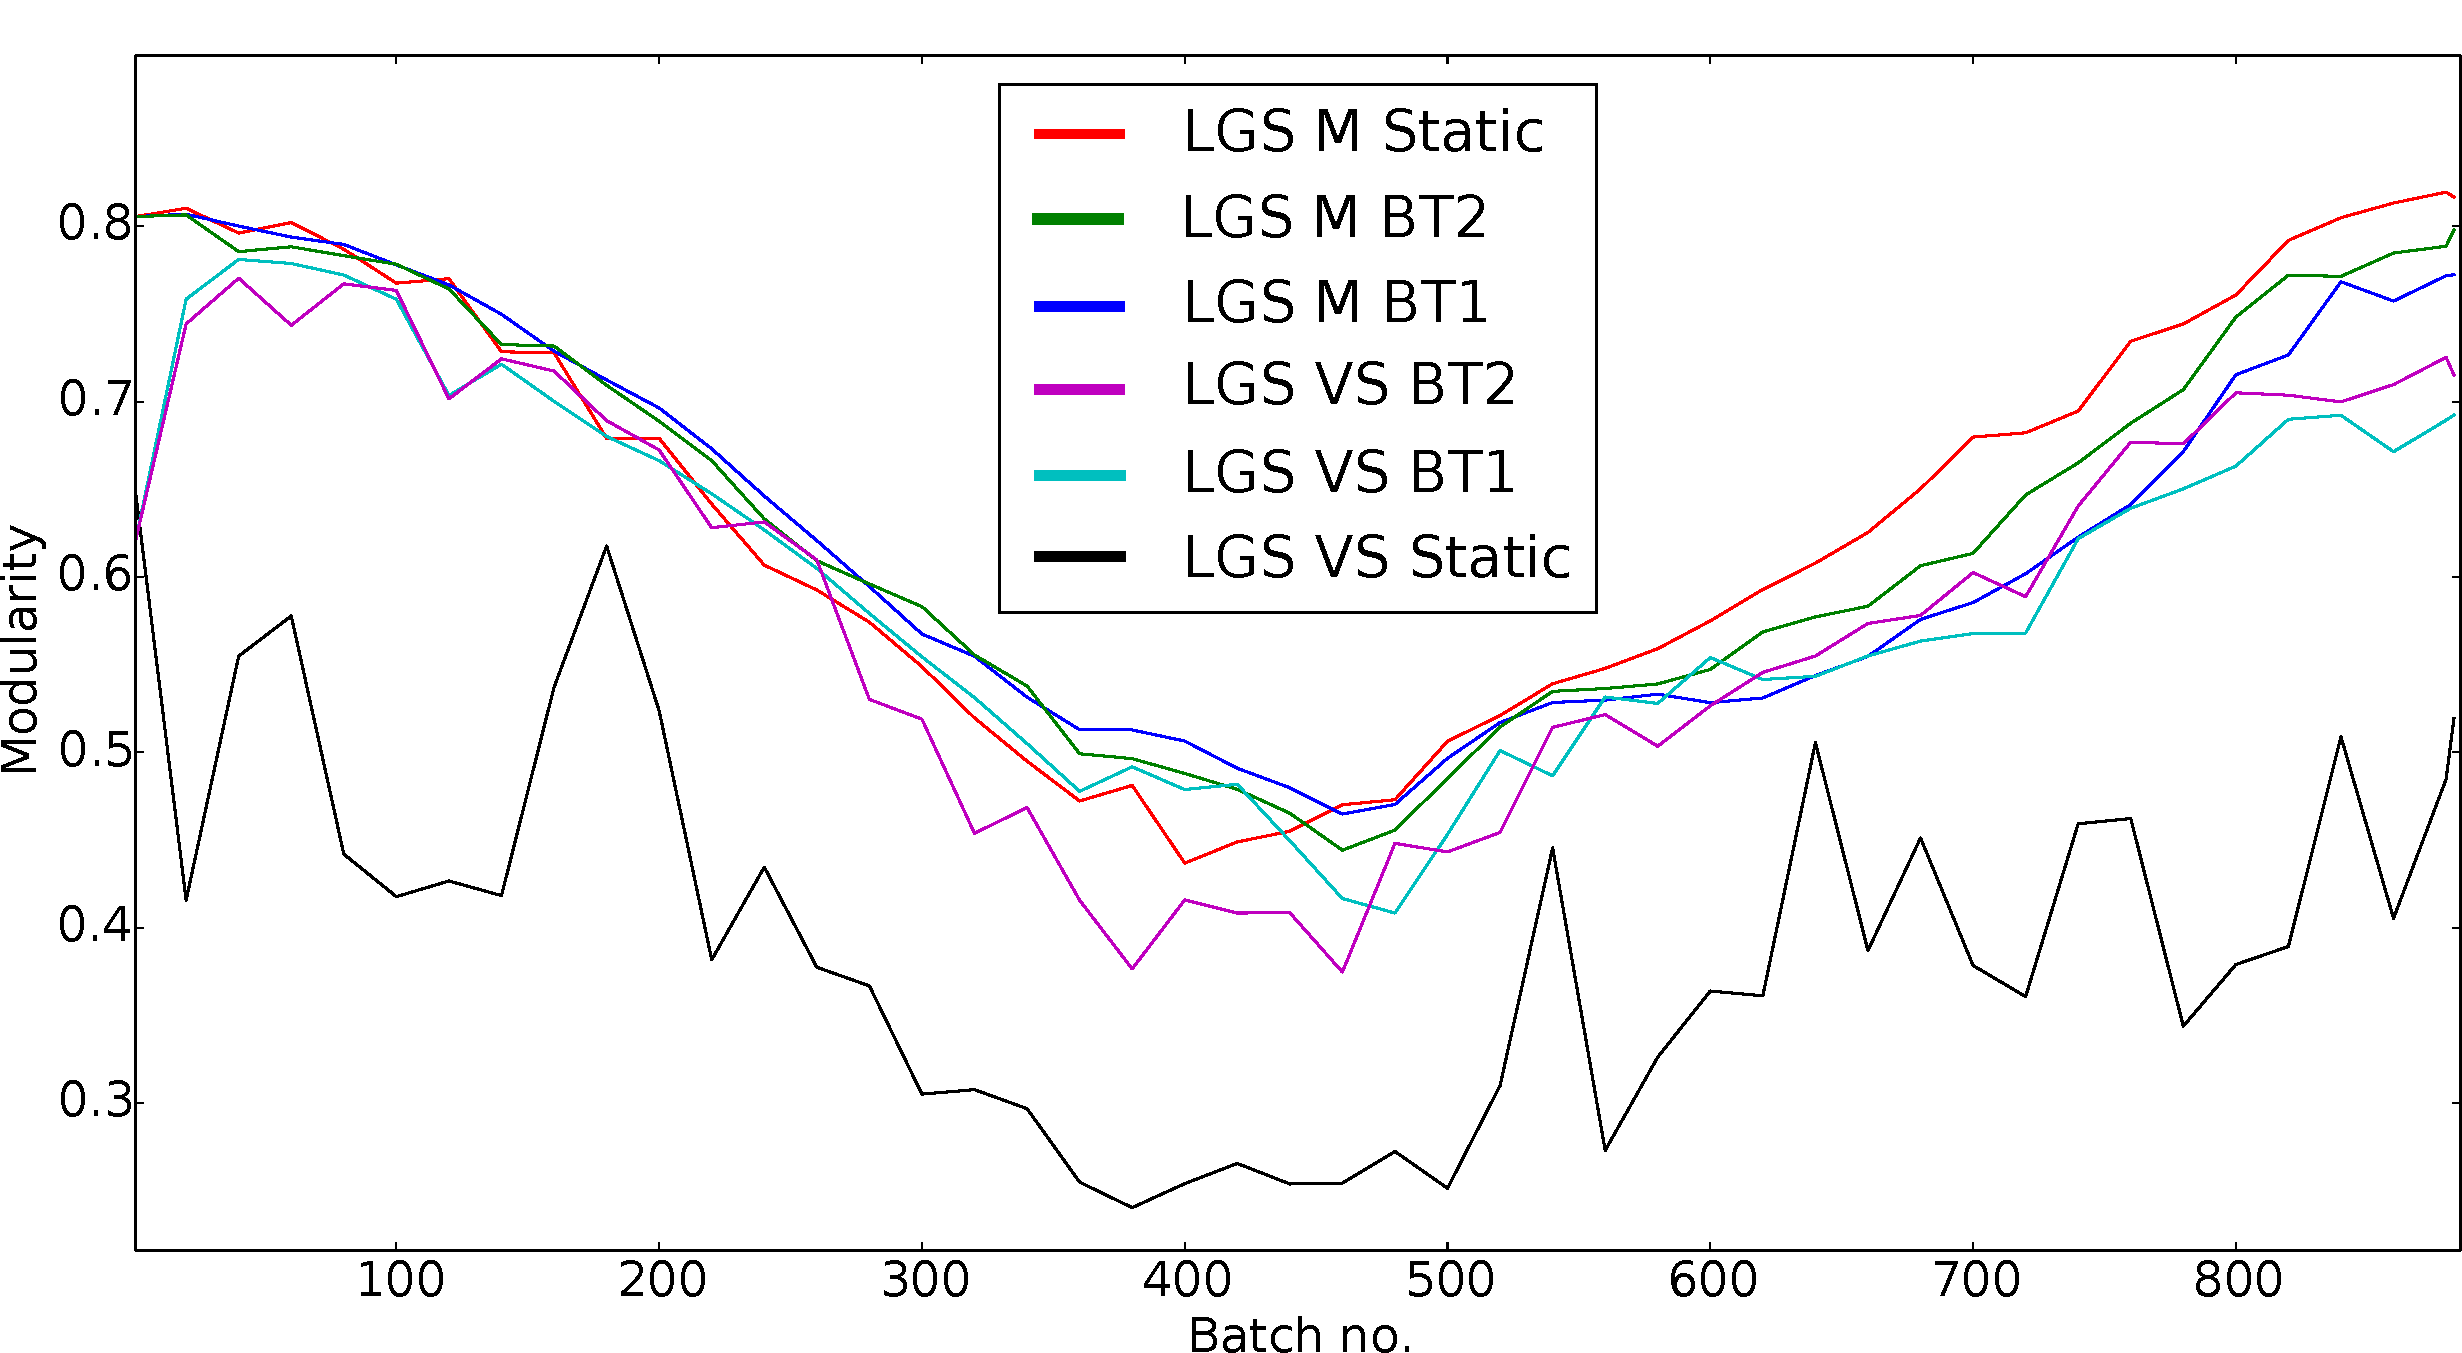
\includegraphics[width=\textwidth]{fb_lgs_mod.pdf}
\vspace{-0.5cm}
\caption{\label{fblgsmod} $G_{fb}$: \emph{Moduarity} evolution for 
Localized Graph Stream\vspace{-0.5cm}}
\end{figure}
\begin{figure}
\centering 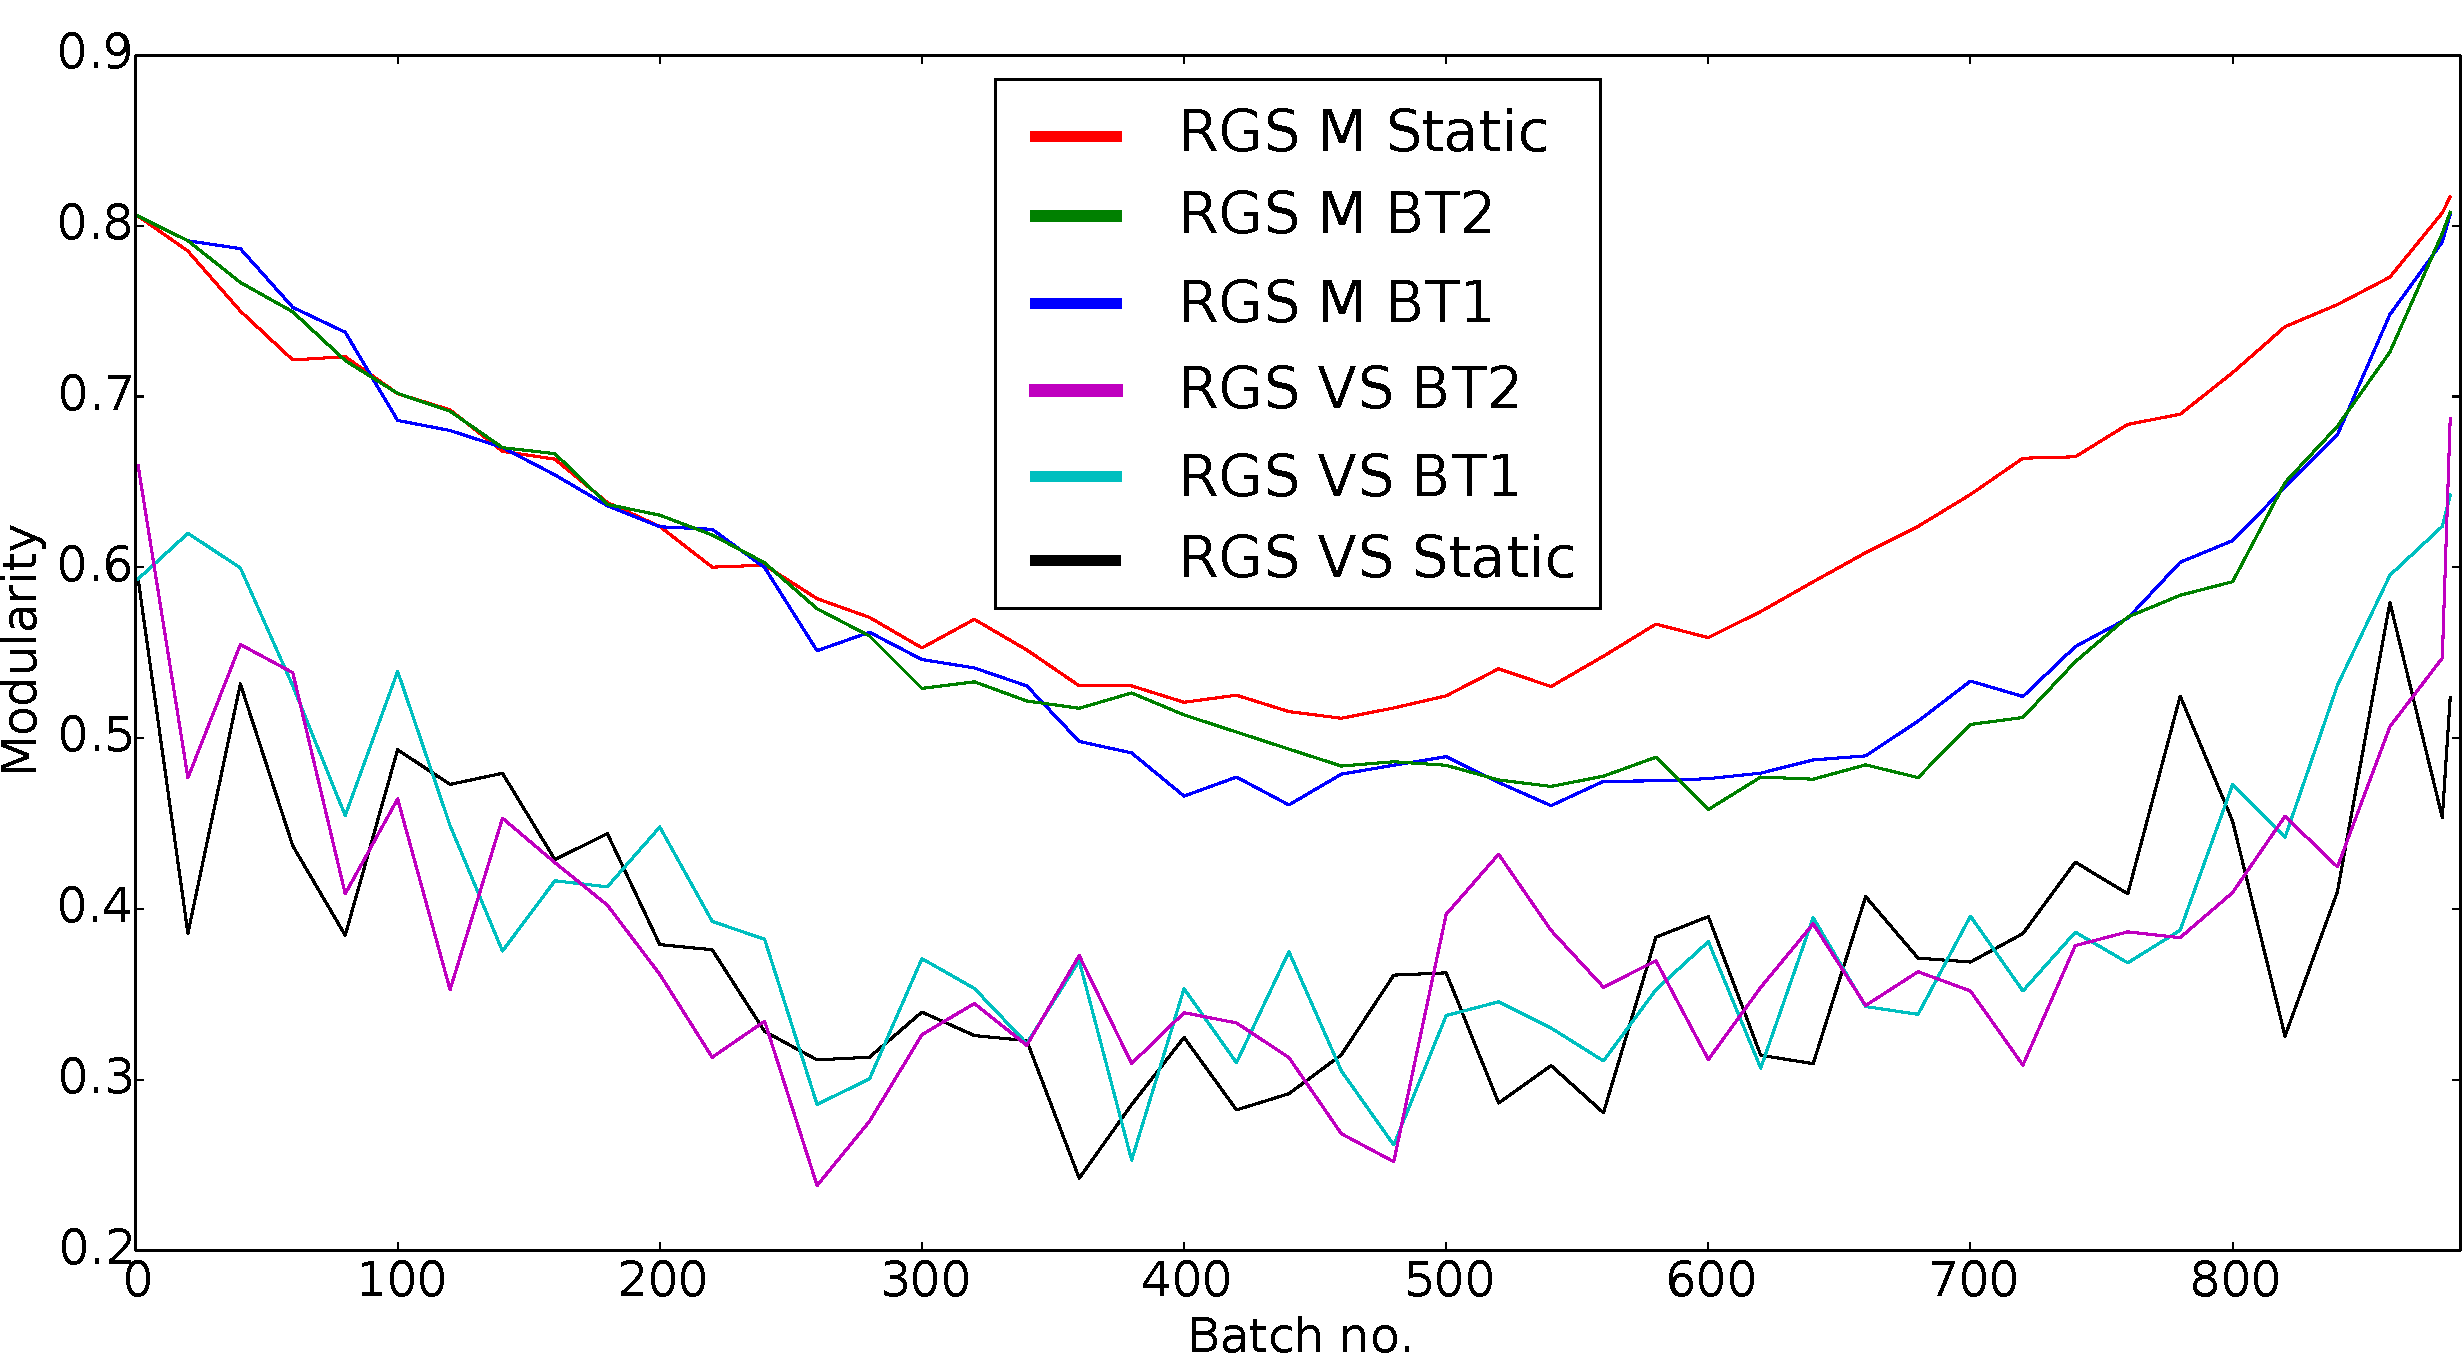
\includegraphics[width=\textwidth]{fb_rgs_mod.pdf}
\vspace{-0.5cm}
\caption{\label{fbrgsmod} $G_{fb}$: \emph{Modularity} evolution for 
Randomized Graph Stream\vspace{-0.6cm}}
\end{figure}
{%
\begin{table}
\newcommand{\mc}[3]{\multicolumn{#1}{#2}{#3}}
\begin{center}
\begin{tabular}{|c|c|c|lll}\cline{1-6}
Modularity & \textit{Initial} & \mc{4}{c|}{\textit{Final}}\\\cline{3-6}
$G_{pgp}$ &  & \mc{2}{c|}{\textit{LGS}} & 
\mc{2}{c|}{\textit{RGS}}\\\cline{3-6}
 & & \textit{Static} & \mc{1}{c|}{\textit{BT1}} & 
\mc{1}{c|}{\textit{Static}} & \mc{1}{c|}{\textit{BT1}}\\\hline
\textit{M} & 0.858 & 0.862 & \mc{1}{c|}{0.857} & \mc{1}{c|}{0.862} & 
\mc{1}{c|}{0.858}\\\hline
\textit{NS} & 0.678 & 0.658 & \mc{1}{c|}{0.779} & \mc{1}{c|}{0.668} & 
\mc{1}{c|}{0.768}\\\hline
\end{tabular}
\end{center}
\vspace{-0.4cm}
\caption{\label{pgpmod}$G_{pgp}$: Modularity}
\end{table}
}%
{%
\begin{table}
\newcommand{\mc}[3]{\multicolumn{#1}{#2}{#3}}
\begin{center}
\begin{tabular}{|c|c|c|ll}\cline{1-5}
$LGS_{fb}$ & Initial & \mc{3}{c|}{Final}\\\cline{3-5}
 &  & M Static & \mc{1}{c|}{M BT1} & \mc{1}{c|}{M BT2}\\\hline
\textit{p} & 12 & 12 & \mc{1}{c|}{8} & \mc{1}{c|}{11}\\\hline
$\mu_{size}$ & 336.58 & 336.58 & \mc{1}{c|}{504.88} & \mc{1}{c|}{367.18}\\\hline
$\sigma_{size}$ & 179.61 & 187.71 & \mc{1}{c|}{359.29} & 
\mc{1}{c|}{213.9}\\\hline
\end{tabular}
\vspace{-0.4cm}
\caption{\label{lgsfbmetrics}$LGS_{fb}$ Key parameters
\emph{[p: No. of communities, $\mu_{size}$: Community size mean, 
$\sigma_{size}$: Community size standard deviation]}\vspace{-0.3cm}}
\end{center}
\end{table}
}%
\subsubsection{Size of Change}
All Dynamic Matching approaches yield a significantly smoother cluster 
transitions with fractional \emph{Size of Change} values compared to the Static 
Matching results as seen in TABLE \ref{soct}, with \emph{BT1} affording lower 
values of than \emph{BT2}, due to higher backtracking in the latter. This 
advantage however is largely lost in the Node Spanning approach with \emph{Size 
of Change} values for Dynamic approaches comparable to Static. This is owing to 
the fact that Node Spanning orders the merges based on an expanding frontier of 
vertices, notwithstanding of the values of \emph{differential modularity}, thus 
following a similar merge order for both Static and Dynamic approaches. A 
significant difference between the two can therefore be observed only if the 
incoming batch of edge-updates drastically modifies the graph, thus creating new 
neighborhoods as can be expected in case of $LGS_{fb}$. Indeed the values of 
\emph{Size of Change} for $NS BT1$ and $NS BT2$ in case of $LGS_{fb}$ are 
significantly lower than that for Static. Finally, under the matching scheme, 
the average \emph{Size of Change} values for LGS can be seen to be considerably 
lower than those for RGS in all cases. This can be attributed to the fact that 
in an edge stream randomized over the graph, the vertices would have a higher 
tendency to jump back and forth across communities during the graph transition. 
Since LGS modifies the graph in a topologically sorted fashion, a region of the 
graph and hence the local clustering would largely remain unchanged once 
updated.
\begin{table}
\begin{center}
\begin{tabular}{|c|c|c|c|c|}\hline
$\mathbf{\nicefrac{\mathbf{Avg\; SOC}}{batch}}$ & \textit{$LGS_{fb}$} & 
\textit{$RGS_{fb}$} & \textit{$LGS_{pgp}$} & \textit{$RGS_{pgp}$}\\\hline
\textit{M Static} & 303 & 457 & 983 & 1205\\\hline
\textit{M BT2} & 97 & 259 & 570 & 817\\\hline
\textit{M BT1} & 74 & 239 & 538 & 772\\\hline
\textit{NS Static} & 559 & 459 & 1161 & 1135\\\hline
\textit{NS BT2} & 127 & 526 & 1080 & 1143\\\hline
\textit{NS BT1} & 76 & 486 & 1032 & 1144\\\hline
\end{tabular}
\vspace{-0.4cm}
\caption{\label{soct}Average \emph{Size of Change} per batch\vspace{-0.1cm}}
\end{center}
\end{table}
\subsubsection{Execution Time}
The critical advantage of dynamic agglomeration becomes evident in the time 
saving over the static approach, as seen in TABLE \ref{ett}. In all cases, the 
trend for execution time follows the order: \emph{M Static} $>$ \emph{M BT2} 
$>$ \emph{M BT1} $>$ \emph{NS Static} $>$ \emph{NS BT2} $>$ \emph{NS BT1}, as 
may be expected from the computation cost. The Node Spanning approaches exhibit 
an order of magnitude improvement over Matching. This advantage is most 
pronounced in case of $LGS_{fb}$ as illustrated in figure \ref{fblgstime}. The 
sudden jumps in execution times of the Dynamic Matching trends show the 
algorithm reacting to a drastic change in the graph.
\begin{figure}
\centering 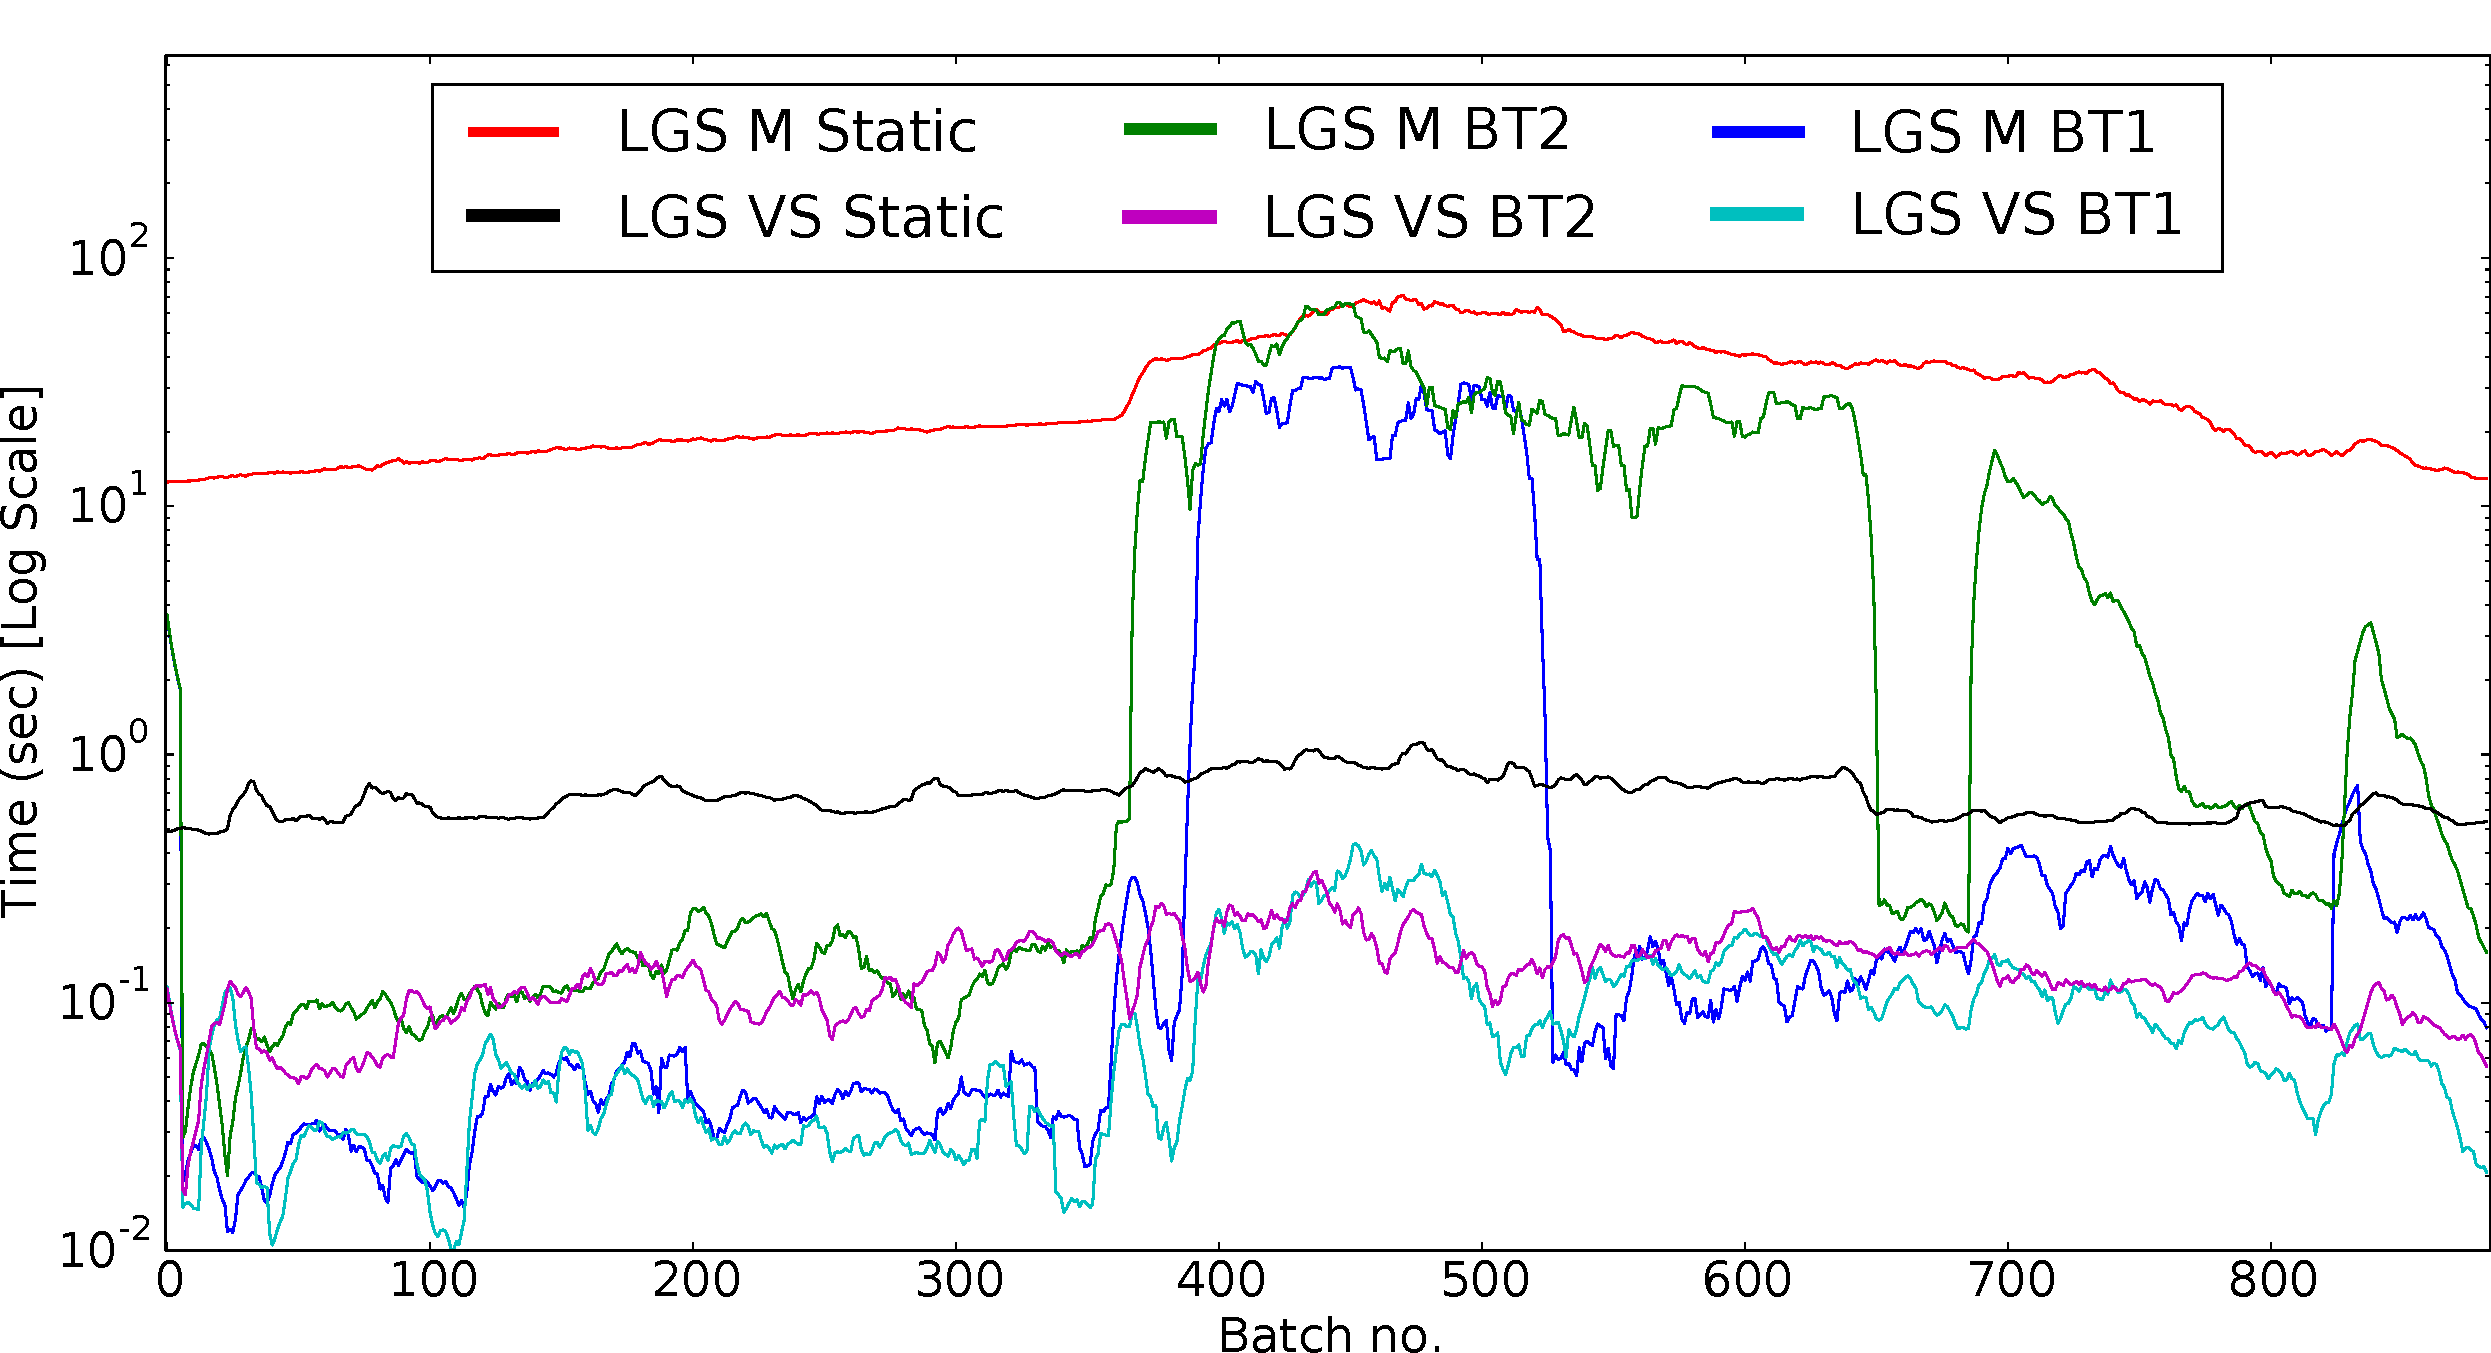
\includegraphics[width=\textwidth]{fb_lgs_time.pdf}
\caption{\label{fblgstime} $G_{fb}$: Execution time/batch 
for Localized Graph Stream\vspace{-0.6cm}}
\end{figure}

\begin{table}
\begin{center}
\begin{tabular}{|c|c|c|c|c|}\hline
$\mathbf{\nicefrac{\mathbf{Avg\; Time}}{batch}}$ & \textit{$LGS_{fb}$} & 
\textit{$RGS_{fb}$} & \textit{$LGS_{pgp}$} & \textit{$RGS_{pgp}$}\\\hline
\textit{M Static} & 29.985 & 19.367 & 1.997 & 1.951\\\hline
\textit{M BT2} & 10.402 & 2.166 & 0.97 & 1.663\\\hline
\textit{M BT1} & 3.872 & 1.199 & 0.92 & 1.517\\\hline
\textit{NS Static} & 0.817 & 0.998 & 1.389 & 1.422\\\hline
\textit{NS BT2} & 0.135 & 0.476 & 0.577 & 0.737\\\hline
\textit{NS BT1} & 0.09 & 0.469 & 0.537 & 0.729\\\hline
\end{tabular}
\vspace{-0.4cm}
\caption{\label{ett}Average execution time per 
batch (seconds)\vspace{-0.5cm}}
\end{center}
\end{table}
Thus we observe that critical trade-offs exists between various agglomeration 
and backtracking schemes. While the Static Matching approach yields the highest 
Modularity values, it performs worst in terms of \emph{Size of Change} and is 
prohibitively slow, especially for high degree graphs such as $G_{fb}$. While 
the Node Spanning based dynamic approaches yield reasonable modularity values, 
within 85\% of those afforded by Static Matching at a small fraction of the 
computational cost, they sacrifice the \emph{Size of Change} in doing so. All 
the dynamic clustering approaches are able to recover, if not exceed the 
initial modularity in transitioning from $G$ to $G^{flip}$, with much relaxed 
backtracking strategies.
\section{Conclusions}
We have presented here a generic framework for a backtracking based dynamic 
reagglomeration algorithm. We demonstrate and evaluate various agglomeration 
and backtracking strategies for realizing the dynamic reagglomeration. The 
dendogram based backtracking technique yields a much more consistent clustering 
compared to the conventional vertex-freeing based dynamic schemes. For
evaluation of the algorithm, we present an objectively testable experiment 
that modifies the graph based on vertex label swapping, while maintaining the 
community structure. Experimental evaluation on $G_{fb}$ \cite{fb} and 
$G_{pgp}$ \cite{pgp} confirms that the dynamic agglomeration approaches perform 
at par if not better than the static approaches in terms of modularity, while 
yielding smoother transitions at fraction of the computation cost, 
particularly in case of high degree graphs such as social networks. The 
analysis reveals that the much economical agglomeration strategies such as 
Matching and Node Spanning; and much relaxed backtracking strategies with 
respect to conventional approaches, perform exceedingly well under dynamic 
clustering.\\
That said, further investigation of the schemes on additional graph data sets 
and stream topologies is necessary to corroborate the presented results. While 
the Matching based agglomeration approach performs better than Node Spanning in 
terms of Modularity and \emph{Size of Change}, the cost of identifying a 
maximum weight matching is fairly high. Further optimization of the Matching 
approach may yield better runtime performance. In that context, because 
matching creates disconnected sets of edges, it makes the matching based 
agglomeration step parallelizable. The subsequent step would be to build on our 
previous work to create a backtracking based parallel agglomeration scheme. 
Finally, further analysis of the backtracking strategies may facilitate the 
implementation of an adaptive backtracking scheme, that determines the suitable 
backtrack policy based on the incoming edge-batch topology.

% \textit{Multi-node spanning:} An extension of this approach would be to span 
% the graph, starting simultaneously from multiple nodes. A special case of this 
% extension would be the all-node spanning approach, wherein all nodes seek out a 
% neighbor to merge with. For a valid merger of two nodes to occur, they would 
% need to seek out each other. The differential modularity information may be 
% used 
% in this case to allow each node to choose the mutually best merge in its 
% neighborhood, thus maximizing the overall improvement in modularity in each 
% step.
% An example of a floating figure using the graphicx package.
% Note that \label must occur AFTER (or within) \caption.
% For figures, \caption should occur after the \includegraphics.
% Note that IEEEtran v1.7 and later has special internal code that
% is designed to preserve the operation of \label within \caption
% even when the captionsoff option is in effect. However, because
% of issues like this, it may be the safest practice to put all your
% \label just after \caption rather than within \caption{}.
%
% Reminder: the "draftcls" or "draftclsnofoot", not "draft", class
% option should be used if it is desired that the figures are to be
% displayed while in draft mode.
%
%\begin{figure}[!t]
%\centering
%\includegraphics[width=2.5in]{myfigure}
% where an .eps filename suffix will be assumed under latex, 
% and a .pdf suffix will be assumed for pdflatex; or what has been declared
% via \DeclareGraphicsExtensions.
%\caption{Simulation results for the network.}
%\label{fig_sim}
%\end{figure}

% Note that the IEEE typically puts floats only at the top, even when this
% results in a large percentage of a column being occupied by floats.


% An example of a double column floating figure using two subfigures.
% (The subfig.sty package must be loaded for this to work.)
% The subfigure \label commands are set within each subfloat command,
% and the \label for the overall figure must come after \caption.
% \hfil is used as a separator to get equal spacing.
% Watch out that the combined width of all the subfigures on a 
% line do not exceed the text width or a line break will occur.
%
%\begin{figure*}[!t]
%\centering
%\subfloat[Case I]{\includegraphics[width=2.5in]{box}%
%\label{fig_first_case}}
%\hfil
%\subfloat[Case II]{\includegraphics[width=2.5in]{box}%
%\label{fig_second_case}}
%\caption{Simulation results for the network.}
%\label{fig_sim}
%\end{figure*}
%
% Note that often IEEE papers with subfigures do not employ subfigure
% captions (using the optional argument to \subfloat[]), but instead will
% reference/describe all of them (a), (b), etc., within the main caption.
% Be aware that for subfig.sty to generate the (a), (b), etc., subfigure
% labels, the optional argument to \subfloat must be present. If a
% subcaption is not desired, just leave its contents blank,
% e.g., \subfloat[].


% An example of a floating table. Note that, for IEEE style tables, the
% \caption command should come BEFORE the table and, given that table
% captions serve much like titles, are usually capitalized except for words
% such as a, an, and, as, at, but, by, for, in, nor, of, on, or, the, to
% and up, which are usually not capitalized unless they are the first or
% last word of the caption. Table text will default to \footnotesize as
% the IEEE normally uses this smaller font for tables.
% The \label must come after \caption as always.
%
%\begin{table}[!t]
%% increase table row spacing, adjust to taste
%\renewcommand{\arraystretch}{1.3}
% if using array.sty, it might be a good idea to tweak the value of
% \extrarowheight as needed to properly center the text within the cells
%\caption{An Example of a Table}
%\label{table_example}
%\centering
%% Some packages, such as MDW tools, offer better commands for making tables
%% than the plain LaTeX2e tabular which is used here.
%\begin{tabular}{|c||c|}
%\hline
%One & Two\\
%\hline
%Three & Four\\
%\hline
%\end{tabular}
%\end{table}


% Note that the IEEE does not put floats in the very first column
% - or typically anywhere on the first page for that matter. Also,
% in-text middle ("here") positioning is typically not used, but it
% is allowed and encouraged for Computer Society conferences (but
% not Computer Society journals). Most IEEE journals/conferences use
% top floats exclusively. 
% Note that, LaTeX2e, unlike IEEE journals/conferences, places
% footnotes above bottom floats. This can be corrected via the
% \fnbelowfloat command of the stfloats package.



% trigger a \newpage just before the given reference
% number - used to balance the columns on the last page
% adjust value as needed - may need to be readjusted if
% the document is modified later
%\IEEEtriggeratref{8}
% The "triggered" command can be changed if desired:
%\IEEEtriggercmd{\enlargethispage{-5in}}

% references section

% can use a bibliography generated by BibTeX as a .bbl file
% BibTeX documentation can be easily obtained at:
% http://mirror.ctan.org/biblio/bibtex/contrib/doc/
% The IEEEtran BibTeX style support page is at:
% http://www.michaelshell.org/tex/ieeetran/bibtex/
%\bibliographystyle{IEEEtran}
% argument is your BibTeX string definitions and bibliography database(s)
%\bibliography{IEEEabrv,../bib/paper}
%
% <OR> manually copy in the resultant .bbl file
% set second argument of \begin to the number of references
% (used to reserve space for the reference number labels box)
\bibliographystyle{IEEEtran}
\bibliography{IEEEabrv,ref}




% that's all folks
\end{document}


